\documentclass[10pt,a4paper]{article}
\usepackage[utf8]{inputenc}
\usepackage[T1]{fontenc}   
\usepackage{amsmath}
\usepackage{amsfonts}
\usepackage{amssymb}
\usepackage{fancyvrb}
\usepackage[left=2cm,right=2cm,top=2cm,bottom=2cm]{geometry}	
\usepackage{msc}
\usepackage{graphicx}

% Setting for MSC diagrams
\setlength{\levelheight}{0.6cm}
\setlength{\instdist}{4.5cm}
\setlength{\actionwidth}{1.5cm}


\author{Lesly-Ann Daniel \and Benjamin Fasquelle \and Rémi Hutin}
\title{SEP challenge}

\setlength\parindent{0pt}

\begin{document}
\maketitle


\section{Protocole}

\begin{itemize}
\item $K$: secret
\item $n$: nonce
\end{itemize}

\begin{table}[!h]
\centering
\begin{tabular}{ll}
$A \rightarrow B:$ & $\langle h(A, K), \{K\}_{pk(B)} \rangle $ \\
$B \rightarrow A:$ & $\langle h(B, K, n), \{n\}_{pk(A)} \rangle $\\
$A \rightarrow B:$ & $h(n)$\\
\end{tabular}
\end{table}

\textbf{Connaissances initiales :} 
Au début du protocole, on suppose que l'agent A connaît la clef publique $pk(B)$ associée à l'agent B,
et que l'agent B connaît la clef publique $pk(A)$ associée à l'agent A. \\

\textbf{Valeurs générées au cours du protocole :} 
$K$ est un secret frais créé par A.
$n$ est un nonce généré par B.\\

\textbf{Description du protocole :}
À la première étape du protocole, l'agent A envoie un hash de son nom et du secret $K$. 
A envoie également un message chiffré contenant le secret $K$. 
Ce dernier est chiffré par un algorithme de chiffrement asymétrique avec la \emph{clef publique} de B, notée $pk(B)$.
Seul l'agent B connaît la clef privée correspondant à la clef publique $pk(B)$. 

À la seconde étape du protocole, l'agent B reçoit le message $\langle h(A, K), \{K\}_{pk(B)} \rangle $, envoyé par l'agent A.
Grâce à sa clef privée, l'agent B peut ouvrir la deuxième partie du message, et donc connaître $K$.
Il peut ensuite calculer le hash de A et $K$ et s'assurer que le secret n'a pas été réutilisé par un attaquant.
Il renvoie alors un hash de son nom, du secret $K$, et d'un nonce $n$, qu'il vient d'engendrer.
Il envoie également le nonce $n$, chiffré avec la clef publique $pk(A)$ de l'agent A.

À la troisième étape du protocole, l'agent A reçoit le message $\langle h(B, K, n), \{n\}_{pk(A)} \rangle $, envoyé par l'agent B.
Grâce à sa clef privée, l'agent A peut ouvrir la deuxième partie du message, et donc connaître $n$.
Il peut aussi s'assurer de l'identité de B puisque seul lui a pu déchiffrer K.
A renvoie alors un hash du nonce $n$. B peut alors vérifier que les messages proviennent bien de A puisque seul lui a pu déchiffrer le nonce.\\


\textbf{Propriétés de sécurité :}
\begin{itemize}
 \item Authentification: Si B termine en pensant avoir reçu une donnée K venant de A, alors A lui a bien envoyé K, et si A termine en ayant envoyé une donnée K à B, alors B a bien reçu K.
 \item Confidentialité: Alice et Bob sont les seuls à connaître le secret K (et le nonce n).
\end{itemize}


\textbf{Poids du protocole :}
\begin{itemize}
\item Règle 1 : $f( \langle h(A, K), \{K\}_{pk(B)} \rangle ) = f ( h(A, K) ) + f ( \{K\}_{pk(B)} ) = (5 + 1 + 1) + (1 + 1) = 9 $
\item Règle 2 : $f(\langle h(B, K, n), \{n\}_{pk(A)} \rangle) = f(h(B, K, n)) + f(\{n\}_{pk(A)}) = (5 + 1 + 1 + 1) + (1 + 1) = 10 $
\item Règle 3 : $f(h(n)) = 5 + 1 = 6$
\end{itemize}

\textbf{Coût total :} $f_{tot} = 9 + 10 + 6 = 25$

\begin{figure}[!ht]
\centering
\begin{msc}{Protocole}
  \declinst{A}{$A$}{}
  \declinst{B}{$B$}{}
  \nextlevel
  \action{secret $K$}{A}
  \nextlevel[2]
  \mess{$\langle h(A, K), \{K\}_{pk(B)} \rangle $}{A}{B}
  \nextlevel
  \action{nonce $n$}{B}
  \nextlevel[2]
  \mess{$\langle h(B, K, n), \{n\}_{pk(A)} \rangle $}{B}{A}
  \nextlevel
  \mess{$h(n)$}{A}{B}
  \nextlevel
\end{msc}
\end{figure}

\newpage

\section{Scyther}
Nous utilisons scyther pour vérifier les propriétés suivantes:
\begin{itemize}
 \item Confidentialité de la clé K vis à vis de A et de B.
 \item Non-injective synchronization (qui implique aussi non-injective agreement et weak-aliveness) qui déclare que les messages reçus ont bien été envoyés par le partenaire et les messages reçus ont bien eté reçus.
\end{itemize}
Les deux propriétés ci-dessus suffisent à assurer que la clé K est secrète et que quand les deux partenaires recoivent le dernier message, ils sont sûrs d'avoir communiqué ensemble et que le contenu des messages envoyés et reçus correspond.
Le code scyther est le suivant:
\begin{Verbatim}[fontsize=\scriptsize]
hashfunction h;
usertype MySecret;

protocol myProtocol(A,B)
{
	role A
	{
		fresh K: MySecret;
		var W: Nonce;

		send_1(A, B, h(A, K), {K}pk(B));
		recv_2(B, A, h(B, K, W), {W}pk(A));
		send_3(A, B, h(W));

		claim_4(A, Secret, K);
		claim_6(A, Nisynch);
	}	
	
	role B
	{
		var V: MySecret;
		fresh n: Nonce;

		recv_1(A, B, h(A, V), {V}pk(B));
		send_2(B, A, h(B, V, n), {n}pk(A));
		recv_3(A, B, h(n));

		claim_5(B, Secret, V);
		claim_7(B, Nisynch);
	}
}
\end{Verbatim}
D'après Scyther, les deux proprietés sont verifiées, voir Figure \ref{fig:scyther_proof}. Notez aussi que chaque claim automatique est aussi vérifié par scyther.
Attention cependant, la propriété de synchronisation non-injective ne garantit pas une protection contre les attaques par rejeu, il faudrait prouver la synchronisation injective.

\begin{figure}[h]
\label{fig:scyther_proof}
\centering
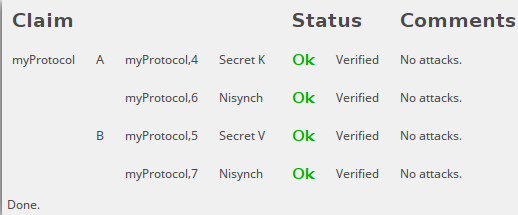
\includegraphics[scale=.5]{scyther_proof}
\caption{Vérification des propriétés par scyther.}
\end{figure}



\section{ProVerif}
La définition des deux processus en \textit{ProVerif} est la suivante:
\begin{Verbatim}[fontsize=\scriptsize]
(* initiator process *)
let Pi(ski:skey, pkr:pkey) = 
  new ki:bitstring;

  (* Send the first message *)
  out(c, (h((pk(ski),ki)), aenc(ki, pkr)));

  (* Receive the second message *)
  in(c, (x1:bitstring, x2:bitstring));
  let (W:bitstring) = adec(x2, ski) in
  (* Check the hash *)
  let (=h((pkr, ki, W)), nr:bitstring) = x1 in

  (* Send the last message*)
  event startI(pk(ski),pkr,ki,W);
  out(c, h(W));
  if pkr <> pk(skc) then
    event acceptI(pk(ski),pkr,ki,W). 

(* responder process *)
let Pr(skr:skey, pki:pkey)=
  (* Receive the first message *)
  in(c, (y1:bitstring, y2:bitstring));
  let (V:bitstring) = adec(y2, skr) in
  let (=h((pki,V))) = y1 in

  (* Send the second message *)
  new nr:bitstring;
  event startR(pki,pk(skr),V,nr);
  out(c, (h((pk(skr), V, nr)), aenc(nr, pki)));

  (* Receive the last message *)
  in(c, y3:bitstring);
  if h(nr) = y3 && pki <> pk(skc) then
    event acceptR(pki,pk(skr),V,nr).
\end{Verbatim}

On ajoute ensuite des queries pour vérifier que K (ki dans \textit{ProVerif}) reste secret:
\begin{Verbatim}[fontsize=\scriptsize]
(* queries *)
query attacker(new ki).

process  ( ! Pi(ska, pk(skb)) | ! Pr(skb, pk(ska))
         | out(c, pk(ska)) | out(c, pk(skb)) | out(c,skc))
\end{Verbatim}
Proverif nour répond que la confidentialité de K est vraie:
\begin{Verbatim}[fontsize=\scriptsize]
-- Query not attacker(ki[!1 = v_417])
Completing...
Starting query not attacker(ki[!1 = v_417])
RESULT not attacker(ki[!1 = v_417]) is true.
\end{Verbatim}

Enfin, pour l'authentification, on définit les propriétés suivantes qui s'assurent que si A termine en ayant envoyé une donnée K à B, alors B a bien reçu K, et si B termine en pensant avoir reçu une donnée K venant de A, alors A lui a bien envoyé K.
\begin{Verbatim}[fontsize=\scriptsize]
(* events *)
event acceptI(pkey, pkey, bitstring, bitstring).
event startR(pkey, pkey, bitstring, bitstring).
event acceptR(pkey, pkey, bitstring, bitstring).
event startI(pkey, pkey, bitstring, bitstring).

(* queries *)
query x1:pkey, x2:pkey, x3:bitstring, x4:bitstring; event(acceptI(x1,x2,x3,x4)) ==> event(startR(x1,x2,x3,x4)).
query x1:pkey, x2:pkey, x3:bitstring, x4:bitstring; event(acceptR(x1,x2,x3,x4)) ==> event(startI(x1,x2,x3,x4)).

(* main process *)
process  ( ! Pi(ska, pk(ska)) | ! Pi(ska, pk(skb)) | ! Pi(ska, pk(skc))
         | ! Pi(skb, pk(ska)) | ! Pi(skb, pk(skb)) | ! Pi(skb, pk(skc))
         | ! Pr(ska, pk(ska)) | ! Pr(ska, pk(skb)) | ! Pr(ska, pk(skc))
         | ! Pr(skb, pk(ska)) | ! Pr(skb, pk(skb)) | ! Pr(skb, pk(skc))
         | out(c, pk(ska)) | out(c, pk(skb)) | out(c,skc)
\end{Verbatim}
\textit{ProVerif} nous répond que nos propriétés sont vraies (pour la seconde propriété, la réponse est similaire):
\begin{Verbatim}[fontsize=\scriptsize]
-- Query event(acceptI(x1_3829,x2_3830,x3_3831,x4_3832)) ==> event(startR(x1_3829,x2_3830,x3_3831,x4_3832))
Completing...
nounif attacker(aenc(V_7143,pk(ska[])))/-5000
200 rules inserted. The rule base contains 141 rules. 96 rules in the queue.
nounif attacker(aenc(V_7387,pk(skb[])))/-5000
Starting query event(acceptI(x1_3829,x2_3830,x3_3831,x4_3832)) ==> event(startR(x1_3829,x2_3830,x3_3831,x4_3832))
goal reachable: begin(startR(pk(skb[]),pk(skb[]),ki_39[!1 = @sid_8579],nr_68[y2_66 = aenc(ki_39[!1 = @sid_8579],pk(skb[])),y1_65 =
h((pk(skb[]),ki_39[!1 = @sid_8579])),!1 = @sid_8580])) -> end(acceptI(pk(skb[]),pk(skb[]),ki_39[!1 = @sid_8579],nr_68[y2_66 =
aenc(ki_39[!1 = @sid_8579],pk(skb[])),y1_65 = h((pk(skb[]),ki_39[!1 = @sid_8579])),!1 = @sid_8580]))
goal reachable: begin(startR(pk(ska[]),pk(skb[]),ki_24[!1 = @sid_8583],nr_63[y2_61 = aenc(ki_24[!1 = @sid_8583],pk(skb[])),y1_60 =
h((pk(ska[]),ki_24[!1 = @sid_8583])),!1 = @sid_8584])) -> end(acceptI(pk(ska[]),pk(skb[]),ki_24[!1 = @sid_8583],nr_63[y2_61 =
aenc(ki_24[!1 = @sid_8583],pk(skb[])),y1_60 = h((pk(ska[]),ki_24[!1 = @sid_8583])),!1 = @sid_8584]))
goal reachable: begin(startR(pk(skb[]),pk(ska[]),ki_34[!1 = @sid_8587],nr_53[y2_51 = aenc(ki_34[!1 = @sid_8587],pk(ska[])),y1_50 =
h((pk(skb[]),ki_34[!1 = @sid_8587])),!1 = @sid_8588])) -> end(acceptI(pk(skb[]),pk(ska[]),ki_34[!1 = @sid_8587],nr_53[y2_51 =
aenc(ki_34[!1 = @sid_8587],pk(ska[])),y1_50 = h((pk(skb[]),ki_34[!1 = @sid_8587])),!1 = @sid_8588]))
goal reachable: begin(startR(pk(ska[]),pk(ska[]),ki[!1 = @sid_8591],nr_49[y2 = aenc(ki[!1 = @sid_8591],pk(ska[])),y1 = h((pk(ska[]),ki[!1 =
@sid_8591])),!1 = @sid_8592])) -> end(acceptI(pk(ska[]),pk(ska[]),ki[!1 = @sid_8591],nr_49[y2 = aenc(ki[!1 = @sid_8591],pk(ska[])),y1 =
h((pk(ska[]),ki[!1 = @sid_8591])),!1 = @sid_8592]))
RESULT event(acceptI(x1_3829,x2_3830,x3_3831,x4_3832)) ==> event(startR(x1_3829,x2_3830,x3_3831,x4_3832)) is true.
\end{Verbatim}
\end{document}
